\input{../utils/preamble}
\createdgmtitle{6}
%--------------------------------------------------------------------------------
\begin{document}
%--------------------------------------------------------------------------------
\begin{frame}
%\thispagestyle{empty}
\titlepage
\end{frame}
%=======
\begin{frame}{RevNets, 2017}
	\begin{minipage}[t]{0.6\columnwidth}
		\begin{itemize}
			\item Modern neural networks are trained via backpropagation.
			\item Residual networks are state of the art in image classification.
			\item Backpropagation requires storing the network activations.
		\end{itemize}
	\end{minipage}%
	\begin{minipage}[t]{0.4\columnwidth}
		\begin{figure}
			\centering
			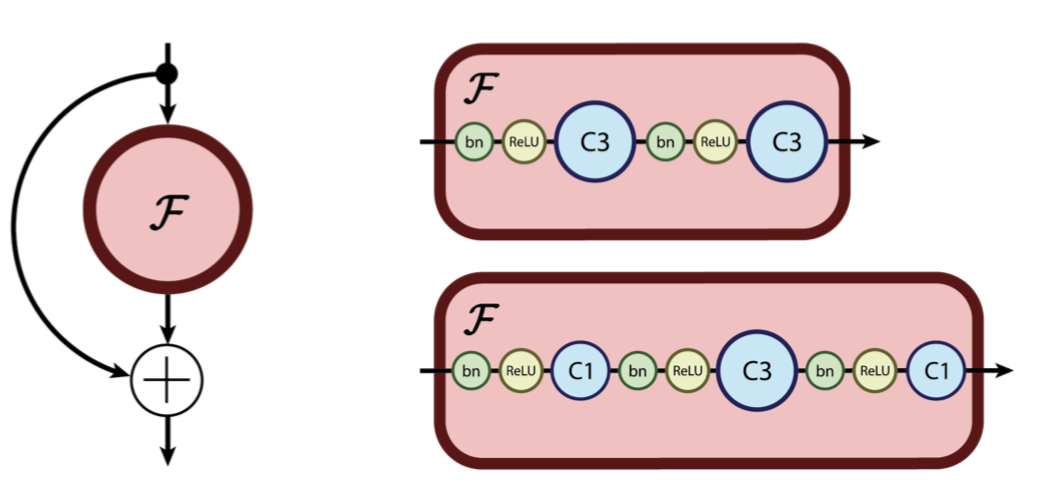
\includegraphics[width=\linewidth]{figs/resnet_block.png}
		\end{figure}
	\end{minipage}
	\vspace{0.1cm}
	\begin{block}{Problem}
		Storing the activations imposes an increasing memory burden. GPUs have limited memory capacity, leading to constraints often exceeded by state-of-the-art architectures (with thousand layers).
	\end{block}
	\myfootnotewithlink{https://arxiv.org/abs/1707.04585}{Gomez A. N. et al. The Reversible Residual Network: Backpropagation Without Storing Activations, 2017}
\end{frame}
%=======
\begin{frame}{RevNets, 2017}
	\begin{block}{NICE}
		\vspace{-0.2cm}
		\begin{equation*}
			\begin{cases} \bz_1 = \bx_1; \\ \bz_2 = \bx_2 + \mathcal{F}(\bx_1, \btheta);\end{cases}  \quad \Leftrightarrow \quad 
			\begin{cases} \bx_1 = \bz_1; \\ \bx_2 = \bz_2 - \mathcal{F}(\bz_1, \btheta).\end{cases} 
		\end{equation*}
		\vspace{-0.2cm}
	\end{block}
	\begin{block}{RevNet}
		\begin{equation*}
			\begin{cases} \by_1 = \bx_1 + \mathcal{F}(\bx_2, \btheta); \\ \by_2 = \bx_2 + \mathcal{G}(\by_1, \btheta);\end{cases} \quad \Leftrightarrow \quad 
			\begin{cases} \bx_2 = \by_2 - \mathcal{F}(\by_1, \btheta); \\ \bx_1 = \by_1 - \mathcal{G}(\bx_2, \btheta).\end{cases} 
		\end{equation*}
	\end{block}
	\begin{figure}
		\centering
		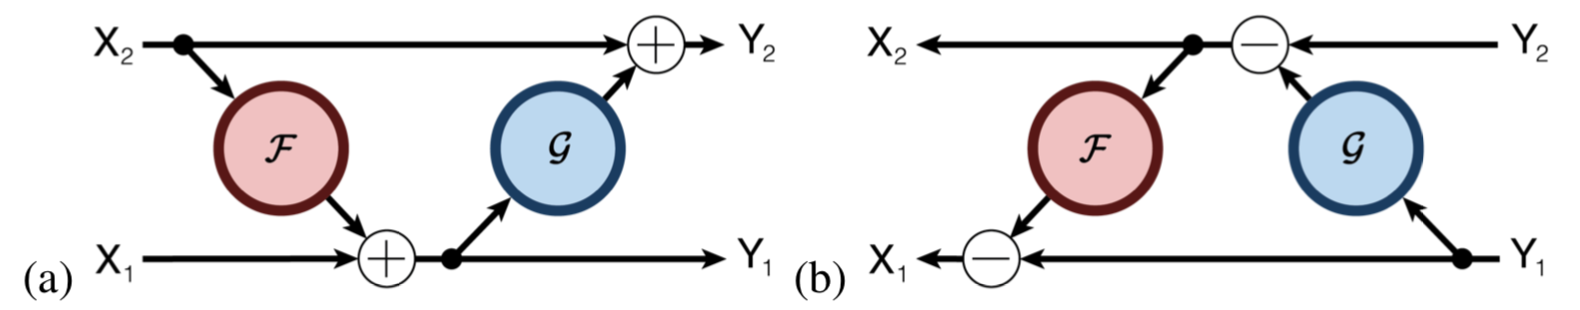
\includegraphics[width=\linewidth]{figs/revnet.png}
	\end{figure}
	\myfootnotewithlink{https://arxiv.org/abs/1707.04585}{Gomez A. N. et al. The Reversible Residual Network: Backpropagation Without Storing Activations, 2017}
\end{frame}
%=======
\begin{frame}{RevNets, 2017}
	\begin{figure}
		\centering
		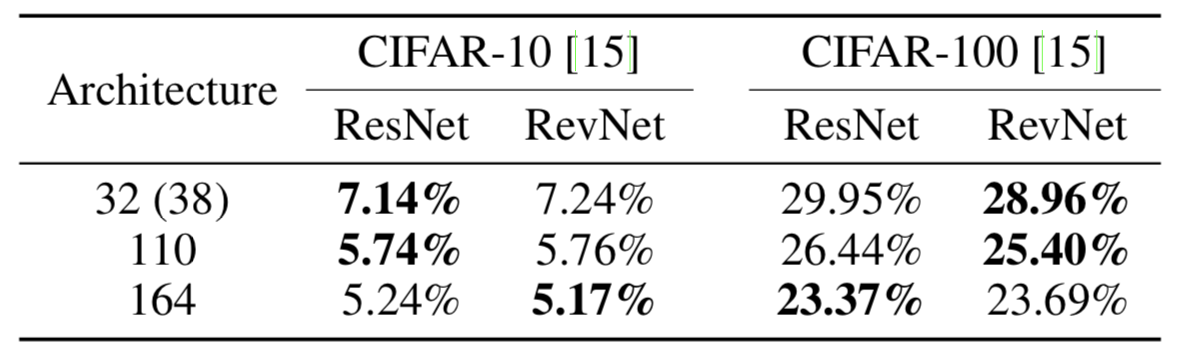
\includegraphics[width=0.8\linewidth]{figs/revnet_results.png}
	\end{figure}
	\begin{itemize}
		\item If the network contains non-reversible blocks (poolings, strides), activations for these blocks should be stored.
		\item To avoid storing activations in the modern frameworks, the backward pass should be manually redefined.
	\end{itemize}
	\myfootnotewithlink{https://arxiv.org/abs/1707.04585}{Gomez A. N. et al. The Reversible Residual Network: Backpropagation Without Storing Activations, 2017}
\end{frame}
%=======
\begin{frame}{i-RevNet, 2018}
	\begin{block}{Hypothesis}
		The success of deep convolutional networks is based on progressively discarding uninformative variability about the input with respect to the problem at hand. 
	\end{block}
	\begin{itemize}
		\item It is difficult to recover images from their hidden representations. 
		\item Information bottleneck principle: an optimal representation must reduce the MI between an input and its representation to reduce uninformative variability + maximize the MI between the output and its representation to preserve each class from collapsing onto other classes.
	\end{itemize}
	\myfootnotewithlink{https://arxiv.org/abs/1802.07088}{Jacobsen J. H., Smeulders A., Oyallon E. i-RevNet: Deep Invertible Networks, 2018}
\end{frame}
%=======
\begin{frame}{i-RevNet, 2018}
	\begin{block}{Hypothesis}
		The success of deep convolutional networks is based on progressively discarding uninformative variability about the input with respect to the problem at hand. 
	\end{block}
	
	\begin{block}{Idea}
		Build a cascade of homeomorphic layers (i-RevNet), a network that can be fully inverted up to the final projection onto the classes, i.e. no information is discarded.
	\end{block}
	\myfootnotewithlink{https://arxiv.org/abs/1802.07088}{Jacobsen J. H., Smeulders A., Oyallon E. i-RevNet: Deep Invertible Networks, 2018}
\end{frame}
%=======
\begin{frame}{i-RevNet, 2018}
	
	\begin{figure}
		\centering
		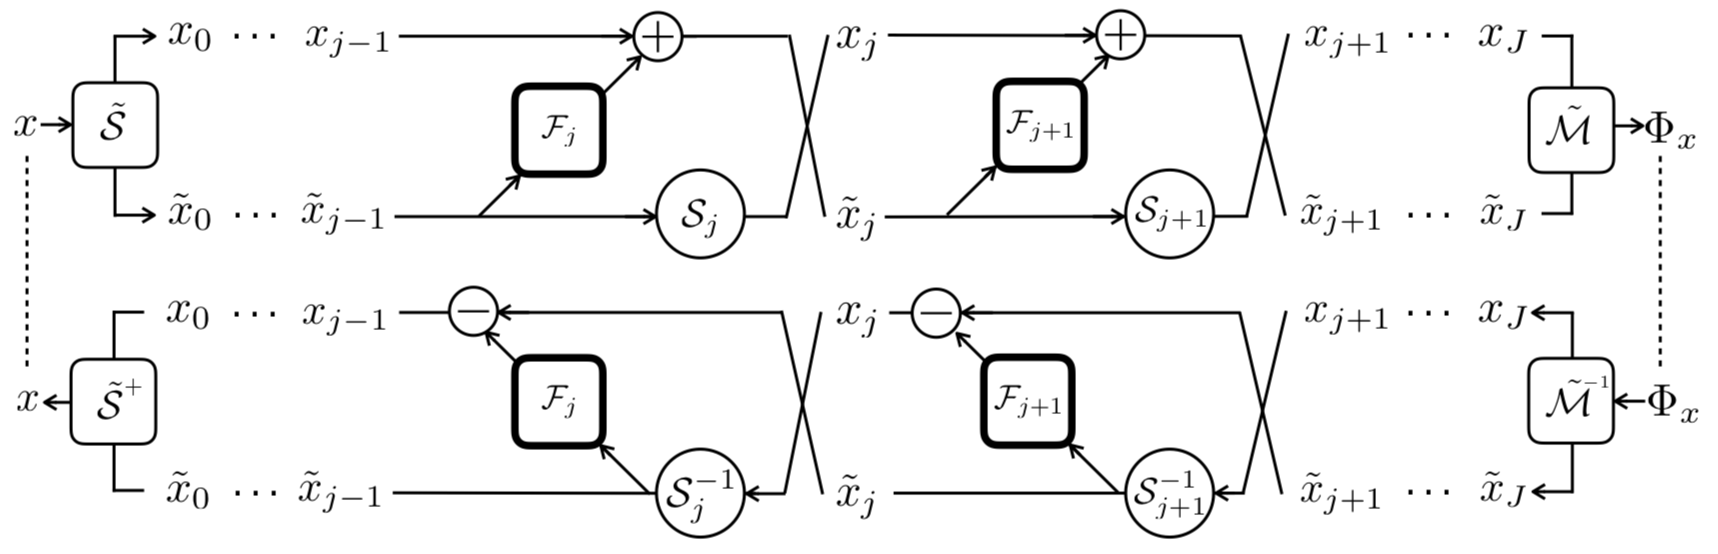
\includegraphics[width=\linewidth]{figs/i-revnet.png}
	\end{figure}
	
	\begin{figure}
		\centering
		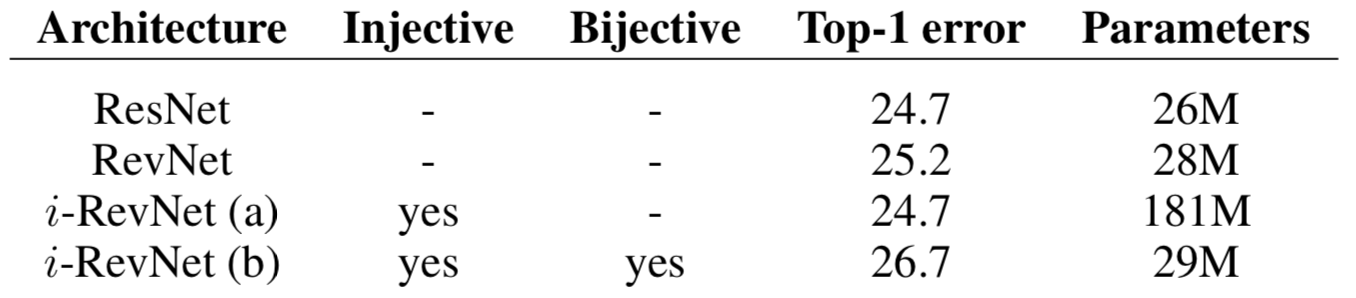
\includegraphics[width=0.9\linewidth]{figs/i-revnet_block.png}
	\end{figure}

	\myfootnotewithlink{https://arxiv.org/abs/1802.07088}{Jacobsen J. H., Smeulders A., Oyallon E. i-RevNet: Deep Invertible Networks, 2018}
\end{frame}
%=======
\begin{frame}{Gaussian autoregressive model}
	Consider autoregressive model
	\[
		p(\bx | \btheta) = \prod_{i=1}^m p(x_i | \bx_{1:i - 1}, \btheta),
	\]
	with conditionals
	\[
	p(x_i | \bx_{1:i - 1}, \btheta) = \mathcal{N} \left(\hat{\mu}_i(\bx_{1:i-1}), \hat{\sigma}^2_i (\bx_{1:i-1})\right).
	\]
	\vspace{-0.5cm}
	\begin{block}{Sampling}
		\[
		x_i = \hat{\sigma}_i (\bx_{1:i-1}) \cdot z_i + \hat{\mu}_i(\bx_{1:i-1}), \quad z_i \sim \mathcal{N}(0, 1).
		\]
	\end{block}
	Sampling from autoregressive model is sequential. \\
	Note that we could interpret this sampling as a transformation $\bx = g(\bz, \btheta)$, where $\bz$ comes from base distribution $\mathcal{N}(0, 1)$.
\end{frame}
%=======
\begin{frame}{Gaussian autoregressive model}
	\begin{block}{Sampling}
		\vspace{-0.5cm}
		\[
		x_i = \hat{\sigma}_i (\bx_{1:i-1}) \cdot z_i + \hat{\mu}_i(\bx_{1:i-1}), \quad z_i \sim \mathcal{N}(0, 1).
		\]
		\vspace{-0.5cm}
	\end{block}
	\begin{block}{Jacobian}
		\vspace{-0.5cm}
		\[
		\log \left|\det \left( \frac{\partial f(\bx, \btheta)}{\partial \bx} \right) \right| = -\log \left|\det \left( \frac{\partial g(\bz, \btheta)}{\partial \bz} \right) \right| = - \sum_{i = 1}^m \log \hat{\sigma}_i (\bx_{1:i-1}).
		\]
		\vspace{-0.5cm}
	\end{block} 
	\begin{block}{Inverse transform}
		\vspace{-0.5cm}
		\[
		z_i = \left(x_i - \hat{\mu}_i(\bx_{1:i-1}) \right) \cdot \frac{1}{\hat{\sigma}_i (\bx_{1:i-1}) }.
		\]
	\end{block}
	We get an autoregressive model with tractable (triangular) Jacobian, which is easily invertible. It is a flow!
\end{frame}
%=======
\begin{frame}{Inverse autoregressive flow (IAF)}
	
	\begin{block}{Gaussian autoregressive model ($\bz \rightarrow \bx$)}
		\vspace{-0.2cm}
		\[
			x_i = \hat{\sigma}_i (\bx_{1:i-1}) \cdot z_i + \hat{\mu}_i(\bx_{1:i-1}).
		\]
		\[
			z_i = \left(x_i - \hat{\mu}_i(\bx_{1:i-1}) \right) \cdot \frac{1}{ \hat{\sigma}_i (\bx_{1:i-1})}.
		\]
		\vspace{-0.3cm}
	\end{block}
	This process is sequential. \\
	Let use the following reparametrization:
	$\bsigma = \frac{1}{\hat{\bsigma}}; \quad \bmu = - \frac{\hat{\bmu}}{\hat{\bsigma}}.$
	
	\begin{block}{Inverse transform ($\bx \rightarrow \bz$)}
		\vspace{-0.2cm}
		\[
			z_i = \sigma_i (\bx_{1:i-1}) \cdot x_i + \mu_i(\bx_{1:i-1}).
		\]
		\[
			x_i = \left( z_i - \mu_i(\bx_{1:i-1})\right) \cdot \frac{1}{\sigma_i (\bx_{1:i-1}) }.
		\]
		\vspace{-0.3cm}
	\end{block}
	This process is \textbf{not} sequential.
	\myfootnotewithlink{https://arxiv.org/abs/1606.04934}{Kingma D. P. et al. Improving Variational Inference with Inverse Autoregressive Flow, 2016} 
\end{frame}
%=======
\begin{frame}{Inverse autoregressive flow (IAF)}
	
	\begin{block}{Inverse transform ($\bx \rightarrow \bz$)}
		\vspace{-0.2cm}
		\[
			z_i = \sigma_i (\bx_{1:i-1}) \cdot x_i + \mu_i(\bx_{1:i-1}).
		\]
		\[
			x_i = \left( z_i - \mu_i(\bx_{1:i-1})\right) \cdot \frac{1}{\sigma_i (\bx_{1:i-1})}.
		\]
		\vspace{-0.3cm}
	\end{block}
	Inverse autoregressive flow use such inverted autoregressive model as a flow in VAE:
	\begin{align*}
		\bz_0 &= \bsigma(\bx) \cdot \bepsilon + \bmu(\bx), \quad \bepsilon \sim \mathcal{N}(0, 1); \quad  \sim q(\bz_0 | \bx, \bphi). \\
		\bz_k &= \bsigma_k(\bz_{k - 1}) \cdot \bz_{k-1} + \bmu_k(\bz_{k - 1}), \quad k \geq 1; \quad  \sim q_k(\bz_k | \bx, \bphi, \{\bphi_j\}_{j=1}^k).
	\end{align*}
	\myfootnotewithlink{https://arxiv.org/abs/1606.04934}{Kingma D. P. et al. Improving Variational Inference with Inverse Autoregressive Flow, 2016} 
\end{frame}
%=======
\begin{frame}{Flows}
	\begin{figure}
		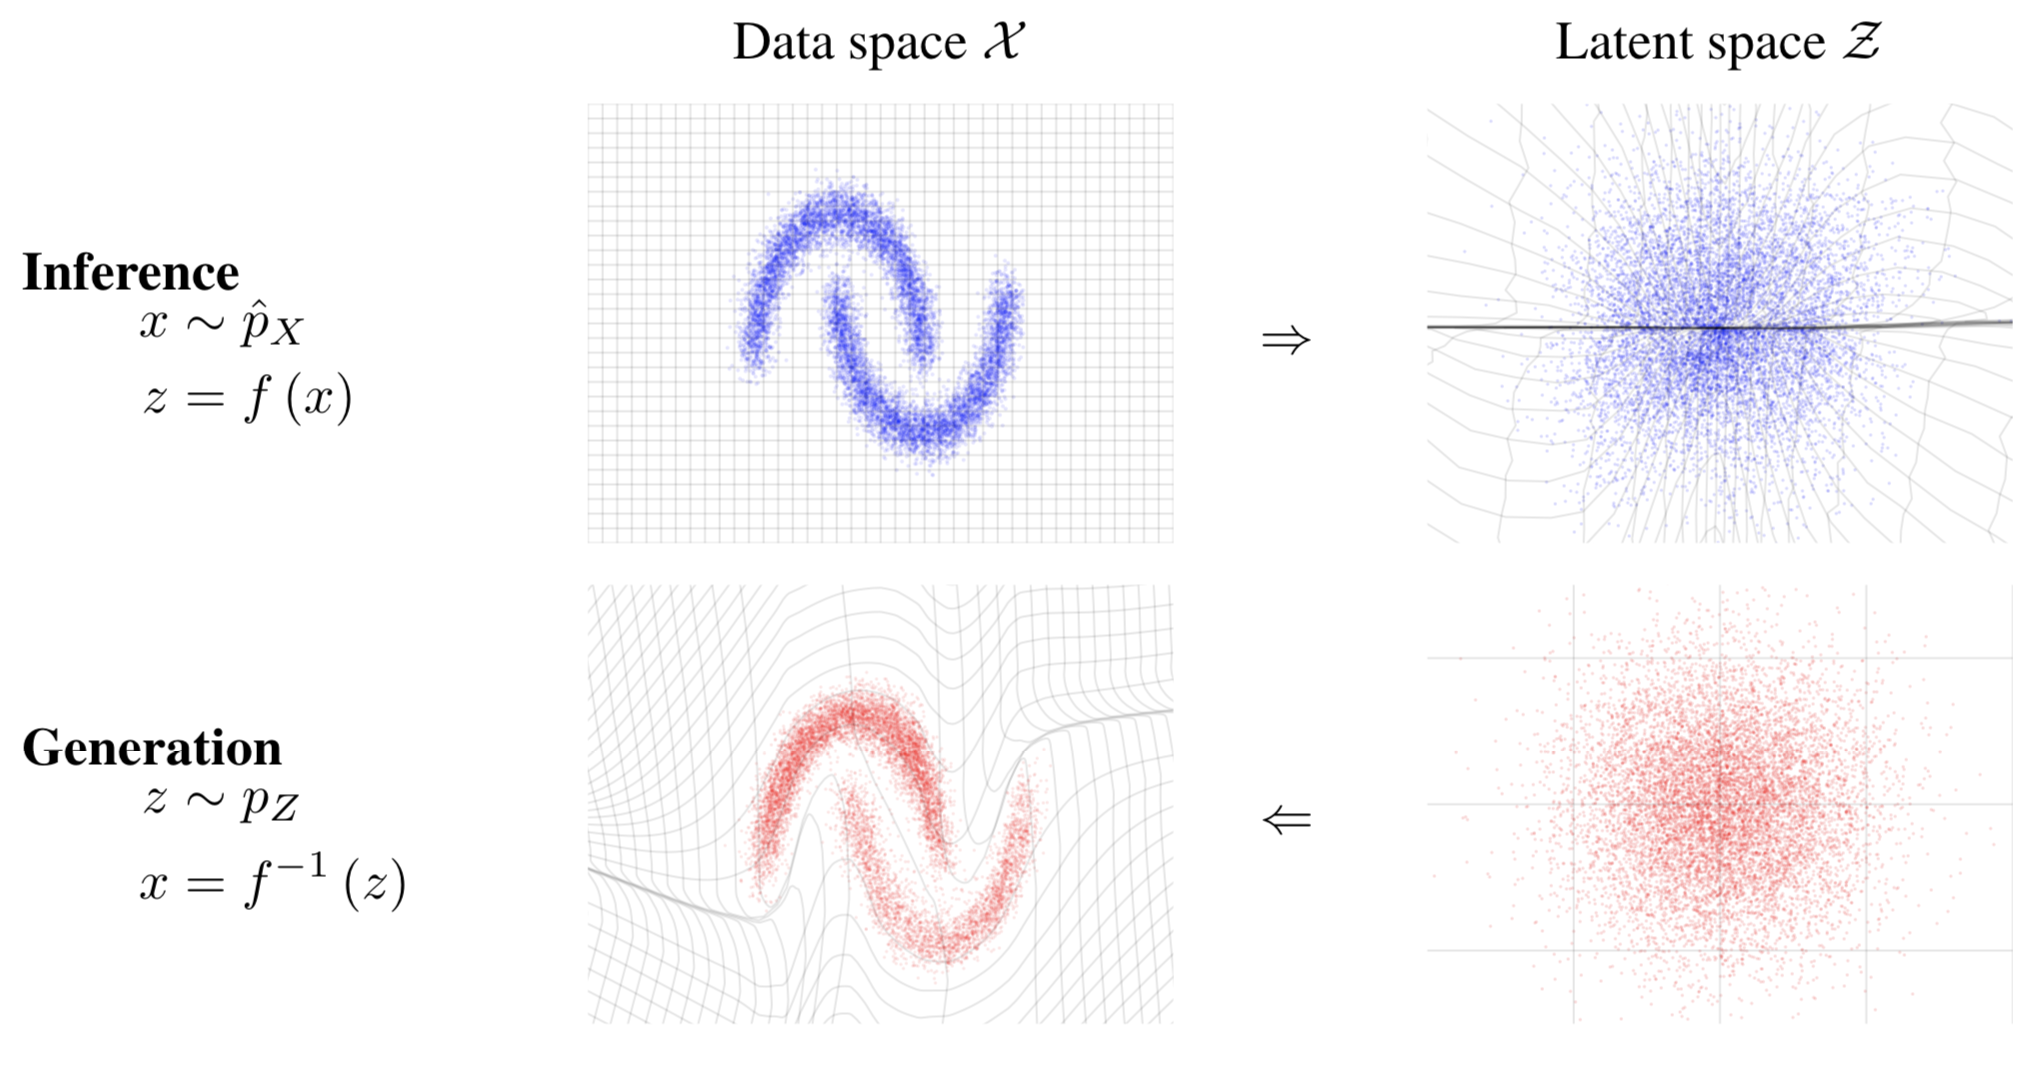
\includegraphics[width=0.8\linewidth]{figs/flows_how2.png}
	\end{figure}
	\begin{itemize}	
		\item Inference mode in autoregressive flows is used for density estimation tasks.
		\item Generation mode in autoregressive flows (IAF) is used for stochastic variational inference to get a more flexible posterior distribution.
	\end{itemize}

	\myfootnotewithlink{https://arxiv.org/abs/1605.08803}{Dinh L., Sohl-Dickstein J., Bengio S. Density estimation using Real NVP, 2016} 
\end{frame}
%=======
\begin{frame}{Inverse autoregressive flow (IAF)}
	\begin{figure}
		\includegraphics[width=\linewidth]{figs/iaf2.png}
	\end{figure}
	\begin{figure}
		\includegraphics[width=\linewidth]{figs/iaf1.png}
	\end{figure}

	\myfootnotewithlink{https://arxiv.org/abs/1606.04934}{Kingma D. P. et al. Improving Variational Inference with Inverse Autoregressive Flow, 2016} 
\end{frame}
%=======
\begin{frame}{Gaussian autoregressive model}
	Consider autoregressive model
	\[
		p(\bx | \btheta) = \prod_{i=1}^m p(x_i | \bx_{1:i - 1}, \btheta),
	\]
	with conditionals
	\[
		p(x_i | \bx_{1:i - 1}, \btheta) = \mathcal{N} \left(\hat{\mu}_i(\bx_{1:i-1}), \hat{\sigma}^2_i (\bx_{1:i-1})\right).
	\]
	\vspace{-0.5cm}
	\begin{block}{Forward and inverse}
		\vspace{-0.3cm}
		\begin{align*}
			x_i &= \hat{\sigma}_i (\bx_{1:i-1}) \cdot z_i + \hat{\mu}_i(\bx_{1:i-1}), \quad z_i \sim \mathcal{N}(0, 1). \\
			z_i &= \left(x_i - \hat{\mu}_i(\bx_{1:i-1}) \right) \cdot \frac{1}{\hat{\sigma}_i (\bx_{1:i-1}) }.
		\end{align*}
	\end{block}
\end{frame}
%=======
\begin{frame}{Gaussian autoregressive model}
	\begin{block}{Forward and inverse}
		\vspace{-0.3cm}
		\begin{align*}
			\bx &= g(\bz, \btheta); \quad x_i = \hat{\sigma}_i (\bx_{1:i-1}) \cdot z_i + \hat{\mu}_i(\bx_{1:i-1}), \quad z_i \sim \mathcal{N}(0, 1). \\
			\bz &= f(\bx, \btheta); \quad z_i = \left(x_i - \hat{\mu}_i(\bx_{1:i-1}) \right) \cdot \frac{1}{\hat{\sigma}_i (\bx_{1:i-1}) }.
		\end{align*}
	\vspace{-0.3cm}
	\end{block}
	\begin{block}{Jacobian}
		\vspace{-0.3cm}
		\[
		\log \left|\det \left( \frac{\partial f(\bx, \btheta)}{\partial \bx} \right) \right| = -\log \left|\det \left( \frac{\partial g(\bz, \btheta)}{\partial \bz} \right) \right| = - \sum_{i = 1}^m \log \hat{\sigma}_i (\bx_{1:i-1}).
		\]
		\vspace{-0.3cm}
	\end{block} 
	We get an autoregressive model with tractable (triangular) Jacobian, which is easily invertible. It is a flow!
\end{frame}
%=======
\begin{frame}{Inverse autoregressive flow (IAF)}
	
	\begin{block}{Gaussian autoregressive model ($\bz \rightarrow \bx$)}
		\vspace{-0.5cm}
		\begin{align*}
		x_i &= \hat{\sigma}_i (\bx_{1:i-1}) \cdot z_i + \hat{\mu}_i(\bx_{1:i-1}).\\
		z_i &= \left(x_i - \hat{\mu}_i(\bx_{1:i-1}) \right) \cdot \frac{1}{ \hat{\sigma}_i (\bx_{1:i-1})}.
		\end{align*}
		\vspace{-0.5cm}
	\end{block}
	This process is sequential. \\
	Let use the following reparametrization:
	$\bsigma = \frac{1}{\hat{\bsigma}}; \quad \bmu = - \frac{\hat{\bmu}}{\hat{\bsigma}}.$
	
	\begin{block}{Inverse transform ($\bx \rightarrow \bz$)}
		\vspace{-0.3cm}
		\begin{align*}
		z_i &= \sigma_i (\bx_{1:i-1}) \cdot x_i + \mu_i(\bx_{1:i-1}). \\
		x_i &= \left( z_i - \mu_i(\bx_{1:i-1})\right) \cdot \frac{1}{\sigma_i (\bx_{1:i-1}) }.
		\end{align*}
		\vspace{-0.3cm}
	\end{block}
	This process is \textbf{not} sequential.

	\myfootnotewithlink{https://arxiv.org/abs/1606.04934}{Kingma D. P. et al. Improving Variational Inference with Inverse Autoregressive Flow, 2016} 
\end{frame}
%=======
\begin{frame}{Inverse autoregressive flow (IAF)}

	\begin{minipage}[t]{0.65\columnwidth}
		\begin{block}{Gaussian autoregressive model}
			\[
			x_i = \hat{\sigma}_i (\bx_{1:i-1}) \cdot z_i + \hat{\mu}_i(\bx_{1:i-1}).
			\]
		\end{block}
	\end{minipage}%
	\begin{minipage}[t]{0.35\columnwidth}
		\begin{figure}[h]
			\centering
			\includegraphics[width=.9\linewidth]{figs/maf_iaf_explained_1.png}
		\end{figure}
	\end{minipage} \\
	
	\begin{minipage}[t]{0.65\columnwidth}
		\begin{block}{Inverse transform}
			\vspace{-0.5cm}
			\begin{align*}
				z_i &= (x_i - \hat{\mu}_i(\bx_{1:i-1})) \cdot \frac{1}{\hat{\sigma}_i (\bx_{1:i-1}) }; \\
				z_i &= \sigma_i (\bx_{1:i-1}) \cdot x_i + \mu_i(\bx_{1:i-1}).
			\end{align*}
			\vspace{-0.4cm}
		\end{block}
	\end{minipage}% 
	\begin{minipage}[t]{0.35\columnwidth}
		\begin{figure}[h]
			\centering
			\includegraphics[width=.9\linewidth]{figs/maf_iaf_explained_2.png}
		\end{figure}
	\end{minipage}\\
	\vspace{0.1cm}
	
	\begin{minipage}[t]{0.65\columnwidth}
		\begin{block}{Inverse autoregressive flow}
			\[
			x_i = \sigma_i (\bz_{1:i-1}) \cdot z_i + \mu_i(\bz_{1:i-1}).
			\]
		\end{block}
	\end{minipage}%
	\begin{minipage}[t]{0.35\columnwidth}
		\begin{figure}[h]
			\centering
			\includegraphics[width=.9\linewidth]{figs/maf_iaf_explained_3.png}
		\end{figure}
	\end{minipage}
	
	\myfootnotewithlink{https://blog.evjang.com/2018/01/nf2.html}{image credit: https://blog.evjang.com/2018/01/nf2.html}
\end{frame}
%=======
\begin{frame}{Flows}
	\begin{figure}
		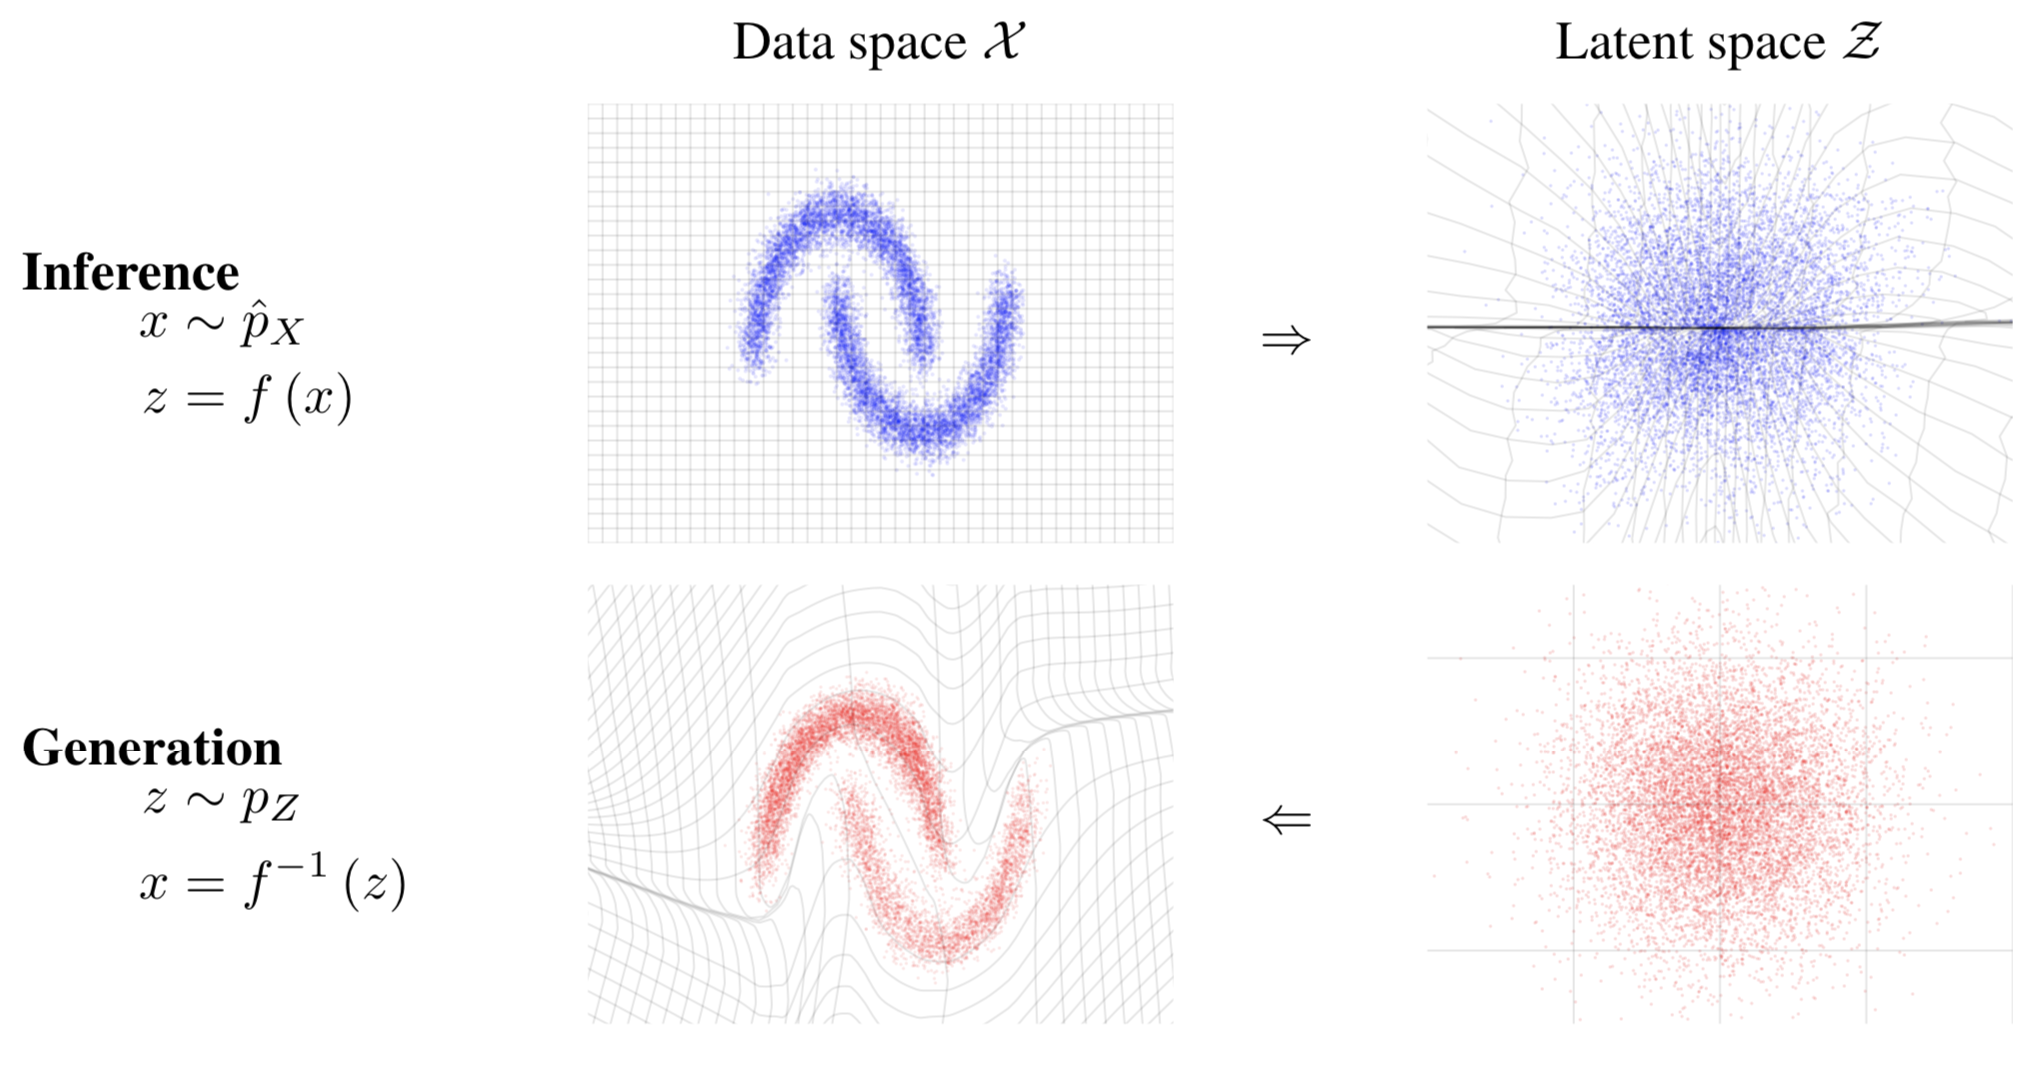
\includegraphics[width=0.8\linewidth]{figs/flows_how2.png}
	\end{figure}
	\begin{itemize}	
		\item Inference mode in autoregressive flows is used for density estimation task.
		\item Generation mode in autoregressive flows (IAF) is used for stochastic variational inference to get more flexible posterior distribution.
	\end{itemize}
	
	\myfootnotewithlink{https://arxiv.org/abs/1605.08803}{Dinh L., Sohl-Dickstein J., Bengio S. Density estimation using Real NVP, 2016} 
\end{frame}
%=======
\begin{frame}{Inverse autoregressive flow (IAF)}
	
	\begin{block}{Inverse transform ($\bx \rightarrow \bz$)}
		\vspace{-0.2cm}
		\[
		z_i = \bsigma_i (\bx_{1:i-1}) \cdot x_i + \bmu_i(\bx_{1:i-1}).
		\]
		\[
		x_i = \left( z_i - \bmu_i(\bx_{1:i-1})\right) \cdot \frac{1}{\bsigma_i (\bx_{1:i-1})}.
		\]
		\vspace{-0.3cm}
	\end{block}
	Inverse autoregressive flow use such inverted autoregressive model as a flow in VAE:
	\[
	\bz_0 = \bsigma(\bx) \cdot \bepsilon + \bmu(\bx), \quad \bepsilon \sim \mathcal{N}(0, 1); \quad  \sim q(\bz_0 | \bx, \bphi).
	\]
	\[
	\bz_k = \bsigma_k(\bz_{k - 1}) \cdot \bz_{k-1} + \bmu_k(\bz_{k - 1}), \quad k \geq 1; \quad  \sim q_k(\bz_k | \bx, \bphi, \{\bphi_j\}_{j=1}^k).
	\]
	
	\myfootnotewithlink{https://arxiv.org/abs/1606.04934}{Kingma D. P. et al. Improving Variational Inference with Inverse Autoregressive Flow, 2016} 
\end{frame}
%=======
\begin{frame}{Inverse autoregressive flow (IAF)}
	\begin{figure}
		\includegraphics[width=\linewidth]{figs/iaf2.png}
	\end{figure}
	\begin{figure}
		\includegraphics[width=\linewidth]{figs/iaf1.png}
	\end{figure}

	\myfootnotewithlink{https://arxiv.org/abs/1606.04934}{Kingma D. P. et al. Improving Variational Inference with Inverse Autoregressive Flow, 2016} 
\end{frame}
%=======
\begin{frame}{Masked autoregressive flow (MAF)}
	\begin{block}{Gaussian autoregressive model}
		\vspace{-0.5cm}
		\[
		p(\bx | \btheta) = \prod_{i=1}^m p(x_i | \bx_{1:i - 1}, \btheta) = \prod_{i=1}^m \mathcal{N} \left(x_i | \mu_i(\bx_{1:i-1}), \sigma^2_i (\bx_{1:i-1})\right).
		\]
		\vspace{-0.5cm}
	\end{block}
	We could use MADE (masked autoencoder) as conditional model. The sampling order could be crucial.
	\begin{figure}
		\includegraphics[width=\linewidth]{figs/maf1.png}
	\end{figure}
	Samples from the base distribution could be an indicator of how good the flow was fitted. \\
	\myfootnotewithlink{https://arxiv.org/abs/1705.07057}{Papamakarios G., Pavlakou T., Murray I. Masked Autoregressive Flow for Density Estimation, 2017} 
\end{frame}
%=======
\begin{frame}{Masked autoregressive flow (MAF)}
	\begin{block}{Gaussian autoregressive model}
		\vspace{-0.5cm}
		\[
		p(\bx | \btheta) = \prod_{i=1}^m p(x_i | \bx_{1:i - 1}, \btheta) = \prod_{i=1}^m \mathcal{N} \left(x_i | \mu_i(\bx_{1:i-1}), \sigma^2_i (\bx_{1:i-1})\right).
		\]
		\vspace{-0.5cm}
	\end{block}
	\begin{figure}
		\includegraphics[width=\linewidth]{figs/maf1.png}
	\end{figure}
	MAF is just a stacked MADE model.
	\myfootnotewithlink{https://arxiv.org/abs/1705.07057}{Papamakarios G., Pavlakou T., Murray I. Masked Autoregressive Flow for Density Estimation, 2017} 
\end{frame}
%=======
\begin{frame}{MAF vs IAF}
	\begin{block}{Sampling and inverse transform in MAF}
		\vspace{-0.2cm}
		\[
		x_i = \hat{\sigma}_i (\bx_{1:i-1}) \cdot z_i + \hat{\mu}_i(\bx_{1:i-1}).
		\]
		\[
		z_i = \left(x_i - \hat{\mu}_i(\bx_{1:i-1}) \right) \cdot \frac{1}{\hat{\sigma}_i (\bx_{1:i-1}) }.
		\]
		\vspace{-0.5cm}
		\begin{itemize}
			\item Sampling is slow (sequential).
			\item Density estimation is fast.
		\end{itemize}
	\end{block}
	\begin{block}{Sampling and inverse transform in IAF}
		\vspace{-0.2cm}
		\[
		x_i = \sigma_i (\bz_{1:i-1}) \cdot z_i + \mu_i(\bz_{1:i-1}).
		\]
		\[
		z_i = \left(x_i - \mu_i(\bz_{1:i-1}) \right) \cdot \frac{1}{\sigma_i (\bz_{1:i-1})}.
		\]
		\vspace{-0.3cm}
		\begin{itemize}
			\item Sampling is fast.
			\item Density estimation is slow (sequential).
		\end{itemize}
	\end{block}
	\myfootnotewithlink{https://arxiv.org/abs/1705.07057}{Papamakarios G., Pavlakou T., Murray I. Masked Autoregressive Flow for Density Estimation, 2017} 
\end{frame}
%=======
\begin{frame}{MAF vs IAF}
	\begin{block}{Theorem}
		Training a MAF with maximum likelihood corresponds to fitting an implicit IAF  with stochastic variational inference where the posterior is taken to be the base density $\pi(\bz)$:
		\[  
		\max_{\btheta} p(\bX | \btheta) \quad \Leftrightarrow \quad \min_{\btheta} KL\left(p(\bz | \btheta) || \pi(\bz)\right).
		\]
		\vspace{-0.5cm}
		\begin{itemize}
			\item $\pi(\bz)$ is a base distribution; $\pi(\bx)$ is a data distribution.
			\item $\bz = f(\bx, \btheta)$~-- MAF model; $\bx = g(\bz, \btheta)$~-- IAF model.
		\end{itemize}
	\end{block}
	\vspace{-0.3cm}
	\[
	\log p(\bz | \btheta) = \log \pi(g(\bz, \btheta)) + \log \left| \det \left( \frac{\partial g(\bz, \btheta)}{\partial \bz}\right) \right|
	\]
	\[
	\log p(\bx | \btheta) = \log \pi(f(\bx, \btheta)) + \log \left| \det \left( \frac{\partial f(\bx, \btheta)}{\partial \bx}\right) \right|
	\]
	\myfootnotewithlink{https://arxiv.org/abs/1705.07057}{Papamakarios G., Pavlakou T., Murray I. Masked Autoregressive Flow for Density Estimation, 2017} 
\end{frame}
%=======
\begin{frame}{MAF vs IAF}
	\begin{block}{Theorem}
		Training a MAF with maximum likelihood corresponds to fitting an implicit IAF  with stochastic variational inference where the posterior is taken to be the base density $\pi(\bz)$:
		\[  
		\max_{\btheta} p(\bX | \btheta) \quad \Leftrightarrow \quad \min_{\btheta} KL\left(p(\bz | \btheta) || \pi(\bz)\right).
		\]
		\vspace{-0.5cm}
	\end{block}
	\begin{block}{Proof}
		\vspace{-0.5cm}
		\begin{multline*}
			KL\left(p(\bz | \btheta) || \pi(\bz) \right) = \mathbb{E}_{p(\bz | \btheta)} \bigl[ \log p(\bz | \btheta) - \log \pi(\bz) \bigr] = \\ 
			= \mathbb{E}_{p(\bz | \btheta)} \left[ \log \pi(g(\bz, \btheta)) + \log \left| \det \left( \frac{\partial g(\bz, \btheta)}{\partial \bz}\right) \right| - \log \pi(\bz) \right] = \\
			= \mathbb{E}_{\pi(\bx)} \left[ \log \pi(\bx) - \log \left| \det \left( \frac{\partial f(\bx, \btheta)}{\partial \bx}\right) \right| - \log \pi(f(\bx, \btheta)) \right].
		\end{multline*}
	\end{block}
	\myfootnotewithlink{https://arxiv.org/abs/1705.07057}{Papamakarios G., Pavlakou T., Murray I. Masked Autoregressive Flow for Density Estimation, 2017} 
\end{frame}
%=======
\begin{frame}{MAF vs IAF}
	\begin{block}{Proof (continued)}
		\vspace{-0.5cm}
		\begin{multline*}
			KL\left(p(\bz | \btheta) || \pi(\bz) \right) = \\
			=  \mathbb{E}_{\pi(\bx)} \left[ \log \pi(\bx) - \log \left| \det \left( \frac{\partial f(\bx, \btheta)}{\partial \bx}\right) \right| - \log \pi(f(\bx, \btheta)) \right] = \\
			= \mathbb{E}_{\pi(\bx)} \bigl[ \log \pi(\bx) - \log p(\bx | \btheta) \bigr] = KL (\pi(\bx) || p(\bx | \btheta)).
		\end{multline*}
		\begin{align*}
			\argmin_{\btheta}  KL (\pi(\bx) || p(\bx | \btheta)) &= \argmin_{\btheta} \mathbb{E}_{\pi(\bx)} \left[ \log \pi(\bx) - \log p(\bx | \btheta) \right] \\
			&= \argmax_{\btheta} \mathbb{E}_{\pi(\bx)} \log p(\bx | \btheta)
		\end{align*}
		Unbiased estimator is MLE:
		\vspace{-0.2cm}
		\[
		\mathbb{E}_{\pi(\bx)} \log p(\bx | \btheta) = \sum_{i=1}^n \log p(\bx_i | \btheta).
		\]
		\vspace{-0.3cm}
	\end{block}
	\myfootnotewithlink{https://arxiv.org/abs/1705.07057}{Papamakarios G., Pavlakou T., Murray I. Masked Autoregressive Flow for Density Estimation, 2017} 
\end{frame}
%=======
\begin{frame}{MAF vs IAF vs RealNVP}
	\begin{block}{MAF}
		\vspace{-0.3cm}
		\[
		\bx = \hat{\bsigma} (\bx) \odot \bz + \hat{\bmu}(\bx).
		\]
		\vspace{-0.5cm}
		\begin{itemize}
			\item Calculating the density $p(\bx | \btheta)$ - 1 pass.
			\item Sampling - $m$ passes.
		\end{itemize}
	\end{block}
	\begin{block}{IAF}
		\vspace{-0.3cm}
		\[
		\bx = \bsigma (\bz) \odot \bz + \bmu(\bz).
		\]
		\vspace{-0.5cm}
		\begin{itemize}
			\item Calculating the density $p(\bx | \btheta)$ - $m$ passes.
			\item Sampling - 1 pass.
		\end{itemize}
	\end{block}
	\begin{block}{RealNVP}
		\vspace{-1cm}
		\begin{align*}
			\bx_{1:d} &= \bz_{1:d}; \\ \bx_{d:m} &= \bz_{d:m} \odot \exp \left(c_1(\bz_{1:d}, \btheta)\right) + c_2(\bx_{1:d}, \btheta).
		\end{align*}
		\vspace{-0.3cm}
	\end{block}
	\myfootnotewithlink{https://arxiv.org/abs/1705.07057}{Papamakarios G., Pavlakou T., Murray I. Masked Autoregressive Flow for Density Estimation, 2017} 
\end{frame}
%=======
\begin{frame}{MAF vs IAF vs RealNVP}
	\begin{block}{RealNVP}
		\vspace{-0.7cm}
		\begin{align*}
			\bx_{1:d} &= \bz_{1:d}; \\ \bx_{d:m} &= \bz_{d:m} \odot \exp \left(c_1(\bz_{1:d}, \btheta)\right) + c_2(\bx_{1:d}, \btheta).
		\end{align*}
		\vspace{-0.8cm}
	\end{block}
	\begin{itemize}
		\item Calculating the density $p(\bx | \btheta)$ - 1 pass.
		\item Sampling - 1 pass.
	\end{itemize}
	
	RealNVP is a special case of MAF and IAF:
	\begin{block}{MAF}
		\vspace{-0.5cm}
		\begin{equation*}
			\begin{cases}
				\hat{\mu}_i  = \hat{\sigma}_i = 0, \, i = 1, \dots, d; \\
				\hat{\mu}_i, \hat{\sigma}_i \text{ -- functions of } \bx_{1:d}, \, i = d+1, \dots, m.
			\end{cases}
		\end{equation*}
		\vspace{-0.3cm}
	\end{block}
	\begin{block}{IAF}
		\vspace{-0.3cm}
		\begin{equation*}
			\begin{cases}
				\mu_i  = \sigma_i = 0, \, i = 1, \dots, d; \\
				\mu_i, \sigma_i \text{ -- functions of } \bz_{1:d}, \, i = d+1, \dots, m.
			\end{cases}
		\end{equation*}
	\end{block}
	\myfootnotewithlink{https://arxiv.org/abs/1705.07057}{Papamakarios G., Pavlakou T., Murray I. Masked Autoregressive Flow for Density Estimation, 2017} 
\end{frame}
%=======
\begin{frame}{MAF/IAF pros and cons}
	\begin{block}{MAF}
		\begin{itemize}
			\item Sampling is slow.
			\item Likelihood evaluation is fast.
		\end{itemize}
	\end{block}
	\begin{block}{IAF}
		\begin{itemize}
			\item Sampling is fast.
			\item Likelihood evaluation is slow.
		\end{itemize}
	\end{block}
	\vspace{0.3cm}
	How to take the best of both worlds?
\end{frame}
%=======
\begin{frame}{WaveNet (2016)}
	Autoregressive model for raw audio waveforms generation
	\vspace{-0.2cm}
	\[
	p(\bx| \btheta) = \prod_{t=1}^T p(x_t|\bx_{1:t-1}, \btheta).
	\]
	\vspace{-0.2cm}
	The model uses causal dilated convolutions.
	\begin{figure}
		\centering
		\includegraphics[width=0.9\linewidth]{figs/wavenet2.png}
	\end{figure}
	\myfootnotewithlink{https://arxiv.org/abs/1609.03499}{Oord A. et al. Wavenet: A generative model for raw audio, 2016}
\end{frame}
%=======
\begin{frame}{Parallel WaveNet, 2017}
	\begin{block}{Previous WaveNet model}
		\begin{itemize}
			\item raw audio is high-dimensional (e.g. 16000 samples per second for 16kHz audio);
			\item WaveNet encodes 8-bit signal with 256-way categorical distribution.
		\end{itemize}
	\end{block}
	\begin{block}{Goal}
		\begin{itemize}
			\item improved fidelity (24kHz instead of 16kHz) $\rightarrow$ increase dilated convolution filter size from 2 to 3;
			\item 16-bit signals $\rightarrow$ mixture of logistics instead of categorical distribution.
		\end{itemize}
	\end{block}
	\myfootnotewithlink{https://arxiv.org/abs/1711.10433}{Oord A. et al. Parallel WaveNet: Fast High-Fidelity Speech Synthesis, 2017}
\end{frame}
%=======
\begin{frame}{Parallel WaveNet, 2017}
	\begin{block}{Probability density distillation}
		\begin{enumerate}
			\item Train usual WaveNet (MAF) via MLE (teacher network).
			\item Train IAF WaveNet model (student network), which attempts to match the probability of its own samples under the distribution learned by the teacher.
		\end{enumerate}
	\end{block}
	\begin{block}{Student objective}
		\[
		KL(p_s || p_t) = H(p_s, p_t) - H(p_s).
		\]
	\end{block}
	More than 1000x speed-up relative to original WaveNet!
	\myfootnotewithlink{https://arxiv.org/abs/1711.10433}{Oord A. et al. Parallel WaveNet: Fast High-Fidelity Speech Synthesis, 2017}
\end{frame}
%=======
\begin{frame}{Parallel WaveNet, 2017}
	\begin{figure}
		\centering
		\includegraphics[width=\linewidth]{figs/parallel_wavenet.png}
	\end{figure}

	\myfootnotewithlink{https://arxiv.org/abs/1711.10433}{Oord A. et al. Parallel WaveNet: Fast High-Fidelity Speech Synthesis, 2017}
\end{frame}
%=======
\begin{frame}{Summary}
	\begin{itemize}
		\item Flows is a continuous model. To use it for discrete distribution, the data should be dequantized.
		\item Original VAE model has lot of limitations. One of them is a restricted class of variational posteriors.
		\item Using flows in a latent space of VAE could give more flexible posterior distribution.
		\item Gaussian autoregressive model is a special type of flow (RealNVP model is a special type of this autoregressive model)
		\item MAF is an example of such model which is suitable for density estimation tasks.
		\item  IAF used the inverse autoregressive transformation for variational inference task.
	\end{itemize}
\end{frame}
%=======
\begin{frame}{VAE limitations}
\begin{itemize}
	\item Poor variational posterior distribution (encoder)
	\[
		q(\bz | \bx, \bphi) = \mathcal{N}(\bz| \bmu_{\bphi}(\bx), \bsigma^2_{\bphi}(\bx)).
	\]
	\item Poor prior distribution
	\[
		p(\bz) = \mathcal{N}(0, \mathbf{I}).
	\]
	\item Poor probabilistic model (decoder)
	\[
		p(\bx | \bz, \btheta) = \mathcal{N}(\bx| \bmu_{\btheta}(\bz), \bsigma^2_{\btheta}(\bz)).
	\]
	\item Loose lower bound
	\[
		p(\bx | \btheta) - \mathcal{L}(q, \btheta) = (?).
	\]
\end{itemize}
\end{frame}
%=======
\begin{frame}{ELBO surgery, 2016}
		\[
			\mathcal{L} (q, \btheta)  = \int q(\bZ | \bX) \log \frac{p(\bX, \bZ | \btheta)}{q(\bZ | \bX)} d\bZ.
		\]
		\vspace{-0.1cm}
	\begin{block}{ELBO interpretations}
	\begin{itemize}
	    \item Evidence minus posterior KL
	    \vspace{-0.1cm}
	    \[
	        \mathcal{L}(q, \btheta) = \log p(\bX | \btheta) - KL(q(\bZ | \bX) || p(\bZ | \bX, \btheta)).
	    \]
	    \item Average negative energy plus entropy
	    \vspace{-0.1cm}
	    \[
	        \mathcal{L}(q, \btheta) = \mathbb{E}_{q(\bZ | \bX)} p(\bX, \bZ | \btheta) + \mathbb{H} \left[q(\bZ | \bX) \right].
	    \]
	    \item Average term-by-term reconstruction minus KL to prior
	    \vspace{-0.1cm}
	    \[
	        \mathcal{L}(q, \btheta) = \frac{1}{n} \sum_{i=1}^n \left[ \mathbb{E}_{q(\bz_i | \bx_i)} \log p(\bx_i | \bz_i, \btheta) - KL(q(\bz_i | \bx_i) || p(\bz_i)) \right].
	    \]
	\end{itemize}
	\end{block}
	
	\myfootnotewithlink{http://approximateinference.org/accepted/HoffmanJohnson2016.pdf}{Hoffman M. D., Johnson M. J. ELBO surgery: yet another way to carve up the variational evidence lower bound, 2016}
\end{frame}
%=======
\begin{frame}{ELBO surgery, 2016}
	\vspace{-0.3cm}
	\[
	    \mathcal{L}(q, \btheta) = \frac{1}{n} \sum_{i=1}^n \left[ \mathbb{E}_{q(\bz_i | \bx_i)} \log p(\bx_i | \bz_i, \btheta) - KL(q(\bz_i | \bx_i) || p(\bz_i)) \right].
	\]
	\vspace{-0.3cm}
	\begin{block}{Theorem}
	\[
	    \frac{1}{n} \sum_{i=1}^n KL(q(\bz_i | \bx_i) || p(\bz_i)) = KL(q(\bz) || p(\bz)) + \mathbb{I}_{q(i, \bz)} [i, \bz],
	\]
	where $i$ is treated as random variable:
	\footnotesize{
	\[
	    q(i, \bz) = q(i) q(\bz | i); \quad p(i, \bz) = p(i) p(\bz); \quad 
	    q(i) = p(i) = \frac{1}{n}; \quad q(\bz | i) = q(\bz | \bx_i).
	\]
	\[
	    q(\bz) = \sum_{i=1}^n q(i, \bz) = \frac{1}{n} \sum_{i=1}^n q(\bz | \bx_i); \quad  \mathbb{I}_{q(i, \bz)} [i, \bz] = \mathbb{E}_{q(i, \bz)} \log \frac{q(i, \bz)}{q(i)q(\bz)}.
	\]
	}
	\end{block}


	\myfootnotewithlink{http://approximateinference.org/accepted/HoffmanJohnson2016.pdf}{Hoffman M. D., Johnson M. J. ELBO surgery: yet another way to carve up the variational evidence lower bound, 2016}
\end{frame}
%=======
\begin{frame}{ELBO surgery, 2016}
	\begin{block}{Theorem}
	\[
	    \frac{1}{n} \sum_{i=1}^n KL(q(\bz_i | \bx_i) || p(\bz_i)) = KL(q(\bz) || p(\bz)) + \mathbb{I}_{q(i, \bz)} [i, \bz].
	\]
	\end{block}
	\begin{block}{Proof}
	\vspace{-0.3cm}
	{\footnotesize
	\begin{multline*}
	    \frac{1}{n} \sum_{i=1}^n KL(q(\bz_i | \bx_i) || p(\bz_i)) = \sum_{i=1}^n \int q(i) q(\bz | i) \log \frac{q(\bz | i)}{p(\bz)} d \bz = \\
	    = \sum_{i=1}^n \int q(i, \bz) \log \frac{q(i, \bz)}{p(\bz)p(i)} d \bz =
	    \int \sum_{i=1}^n q(i, \bz) \log \frac{ q (\bz) q(i | \bz) }{p(\bz) p(i) } d \bz = \\
	    = \int q(\bz) \log \frac{q(\bz)}{p(\bz)} d\bz + \int \sum_{i=1}^n q(i | \bz) q(\bz) \log \frac{q(i | \bz)}{p(i)} d \bz = \\
	    = KL (q(\bz) || p(\bz)) - \mathbb{E}_{q(\bz)} \mathbb{H} \left[q(i | \bz)  \right] + \log n.
	\end{multline*}
	}
	\end{block}

	\myfootnotewithlink{http://approximateinference.org/accepted/HoffmanJohnson2016.pdf}{Hoffman M. D., Johnson M. J. ELBO surgery: yet another way to carve up the variational evidence lower bound, 2016}
\end{frame}
%=======
\begin{frame}{ELBO surgery, 2016}
	\begin{block}{Theorem}
	\[
	    \frac{1}{n} \sum_{i=1}^n KL(q(\bz_i | \bx_i) || p(\bz_i)) = KL(q(\bz) || p(\bz)) + \mathbb{I}_{q(i, \bz)} [i, \bz].
	\]
	\end{block}
	\begin{block}{Proof (continued)}
	{\footnotesize
	\[
	    \frac{1}{n} \sum_{i=1}^n KL(q(\bz_i | \bx_i) || p(\bz_i)) = KL (q(\bz) || p(\bz)) - \mathbb{E}_{q(\bz)} \mathbb{H} \left[q(i | \bz) \right] + \log n
	\]
	\begin{multline*}
	    \mathbb{I}_{q(i, \bz)} [i, \bz] = \mathbb{E}_{q(i, \bz)} \log \frac{q(i, \bz)}{q(i)q(\bz)} = \mathbb{E}_{q(\bz)} \mathbb{E}_{q(i | \bz)} \log \frac{q(i | \bz) q(\bz)}{q(i)q(\bz)} = \\
	    = \mathbb{E}_{q(\bz)} \mathbb{E}_{q(i | \bz)} \log \frac{q(i | \bz)}{q(i)} = - \mathbb{E}_{q(\bz)} \mathbb{H} \left[ q(i | \bz) \right] + \log n.
	\end{multline*}
	}
	\end{block}

	\myfootnotewithlink{http://approximateinference.org/accepted/HoffmanJohnson2016.pdf}{Hoffman M. D., Johnson M. J. ELBO surgery: yet another way to carve up the variational evidence lower bound, 2016}
\end{frame}
%=======
\begin{frame}{ELBO surgery, 2016}
	\begin{block}{Theorem}
	\[
	    \frac{1}{n} \sum_{i=1}^n KL(q(\bz_i | \bx_i) || p(\bz_i)) = KL(q(\bz) || p(\bz)) + \mathbb{I}_{q(i, \bz)} [i, \bz].
	\]
	\end{block}
	\begin{block}{ELBO revisiting}
	{\footnotesize
	\begin{multline*}
	    \mathcal{L}(q, \btheta) = \frac{1}{n} \sum_{i=1}^n \left[ \mathbb{E}_{q(\bz_i | \bx_i)} \log p(\bx_i | \bz_i, \btheta) - KL(q(\bz_i | \bx_i) || p(\bz_i)) \right] = \\
	    = \frac{1}{n} \sum_{i=1}^n \mathbb{E}_{q(\bz_i | \bx_i)} \log p(\bx_i | \bz_i, \btheta) - \mathbb{I}_{q(i, \bz)} [i, \bz] - KL(q(\bz) || p(\bz)) = \\
	    = \underbrace{\frac{1}{n} \sum_{i=1}^n \mathbb{E}_{q(\bz_i | \bx_i)} \log p(\bx_i | \bz_i, \btheta)}_{\text{Reconstruction loss}} - \underbrace{\left(\log n - \mathbb{E}_{q(\bz)} \mathbb{H} \left[ q(i | \bz) \right] \right)\vphantom{\sum_{i=1}} }_{0 \leq \text{Mutual info} \leq \log n } - \underbrace{KL(q(\bz) || p(\bz))\vphantom{\sum_{i=1}}}_{\text{Marginal KL}}
	\end{multline*}
	}
	\end{block}

	\myfootnotewithlink{http://approximateinference.org/accepted/HoffmanJohnson2016.pdf}{Hoffman M. D., Johnson M. J. ELBO surgery: yet another way to carve up the variational evidence lower bound, 2016}
\end{frame}
%=======
\begin{frame}{ELBO surgery, 2016}
	\begin{block}{ELBO revisiting}
	\vspace{-0.3cm}
	{\footnotesize
	\[
	    \mathcal{L}(q, \btheta) = \underbrace{\frac{1}{n} \sum_{i=1}^n \mathbb{E}_{q(\bz_i | \bx_i)} \log p(\bx_i | \bz_i, \btheta)}_{\text{Reconstruction loss}} - \underbrace{\left(\log n - \mathbb{E}_{q(\bz)} \mathbb{H} \left[ q(i | \bz) \right] \right)\vphantom{\sum_{i=1}}}_{0 \leq \text{Mutual info} \leq \log n } - \underbrace{KL(q(\bz) || p(\bz))\vphantom{\sum_{i=1}}}_{\text{Marginal KL}}
	\]}
	\end{block}
	\vspace{-0.3cm}
	\[
	    KL(q(\bz) || p(\bz)) = 0 \quad \Leftrightarrow \quad p (\bz) = q(\bz) = \frac{1}{n} \sum_{i=1}^n q(\bz | \bx_i).
	\]
	\begin{figure}
	    \centering
	    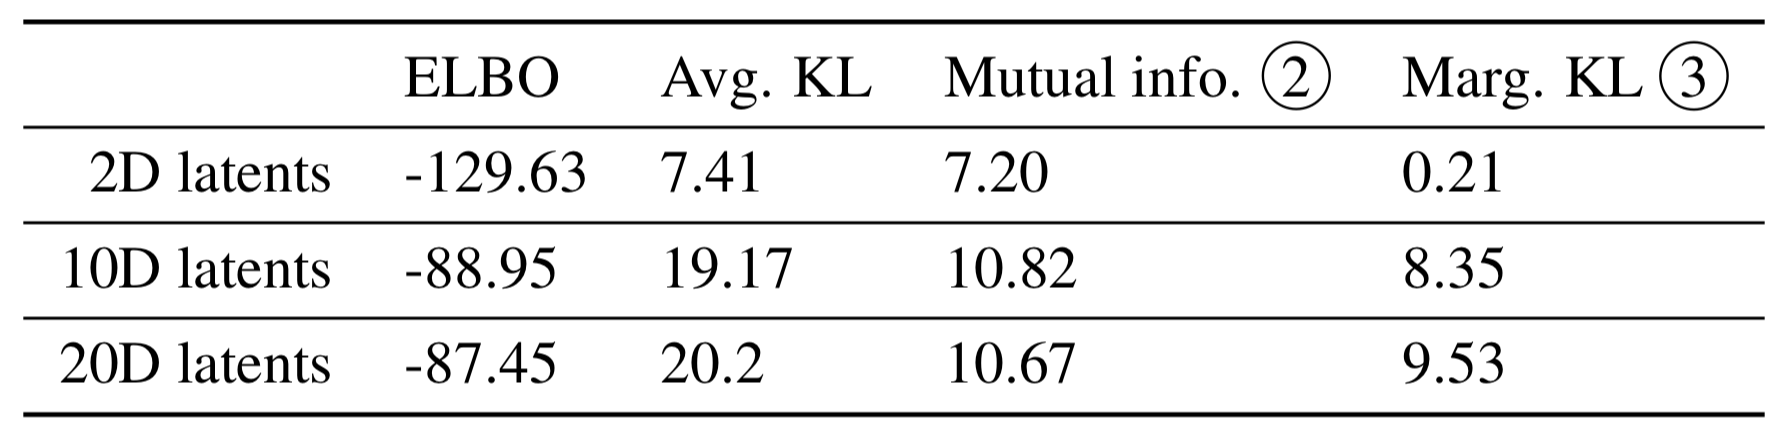
\includegraphics[width=0.8\linewidth]{figs/ELBO_surgery.png}
	\end{figure}
	\[
	\log n \approx 11.0021
	\]

	\myfootnotewithlink{http://approximateinference.org/accepted/HoffmanJohnson2016.pdf}{Hoffman M. D., Johnson M. J. ELBO surgery: yet another way to carve up the variational evidence lower bound, 2016}
\end{frame}
%=======
\begin{frame}{VAE prior}
	\begin{block}{ELBO revisiting}
	\vspace{-0.3cm}
	{\footnotesize
	\[
	    \mathcal{L}(q, \btheta) = \underbrace{\frac{1}{n} \sum_{i=1}^n \mathbb{E}_{q(\bz_i | \bx_i)} \log p(\bx_i | \bz_i, \btheta)}_{\text{Reconstruction loss}} - \underbrace{\left(\log n - \mathbb{E}_{q(\bz)} \mathbb{H} \left[ q(i | \bz) \right] \right)\vphantom{\sum_{i=1}}}_{0 \leq \text{Mutual info} \leq \log N } - \underbrace{KL(q(\bz) || p(\bz))\vphantom{\sum_{i=1}}}_{\text{Marginal KL}}
	\]}
	\end{block}
	
	How to choose the optimal $p(\bz)$?
	\begin{itemize}
	    \item SG: $p(\bz) = \mathcal{N}(0, I)$ $\Rightarrow$ over-regularization;
	    \vspace{0.1cm}
	    \item MoG: $p(\bz | \blambda) = \frac{1}{K} \sum_{k=1}^K \mathcal{N}(\bmu_k, \bsigma_k^2)$ $\Rightarrow$ (*), (**);
	    \vspace{0.1cm}
	    \item $p(\bz) = q(\bz) = \frac{1}{n}\sum_{i=1}^n q(\bz | \bx_i)$ $\Rightarrow$ overfitting and highly expensive.
	\end{itemize}

	\myfootnote{\href{https://arxiv.org/abs/1611.02648}{(*) Dilokthanakul N. et al. Deep Unsupervised Clustering with Gaussian Mixture Variational Autoencoders, 2016} \\
	\href{https://pdfs.semanticscholar.org/f6fe/5e8e25994c188ba6a124462e2cc55f2c5a67.pdf}{(**) Nalisnick E., Hertel L., Smyth P. Approximate Inference for Deep Latent Gaussian Mixtures, 2016}}

\end{frame}
%=======
\begin{frame}{Summary}
\end{frame}
\end{document} 